\chapter{Desenvolvimento e Implementação}
\label{ch::implement}

\section{Introdução}
\label{sec::implement:intro}

Este capítulo explora o percurso realizado aquando do desenvolvimento do projeto descrito neste documento, em particular as escolhas e detalhes de implementação.


\section{Escolhas de Implementação}
\label{sec::implement:struct}

Antes da implementação dos algoritmos para satisfazer as respostas às perguntas colocadas, foi necessário definir a estrutura de dados utilizada para a manipulação do mundo virtual e dos objetos nele contidos.

Desta forma, além da escolha do uso de listas para guardar os objetos que o dispositivo robótico encontra no seu mundo virtual (Figura \ref{fig::hospital}), foi utilizada numa primeira abordagem uma matriz $800\times600$ para efeitos de aplicação de um algoritmo de \textit{path-finding} (necessário para as respostas aos enunciados descritos nas subseccções \ref{ssec::implement:details:perg3}, \ref{ssec::implement:details:perg4} e \ref{ssec::implement:details:perg5}). Esta abordagem revelou alguns problemas de eficiência, conforme é refletido na secção \ref{sec::reflexao:problemas}).

\begin{figure}[!hbtp]
    \centering
    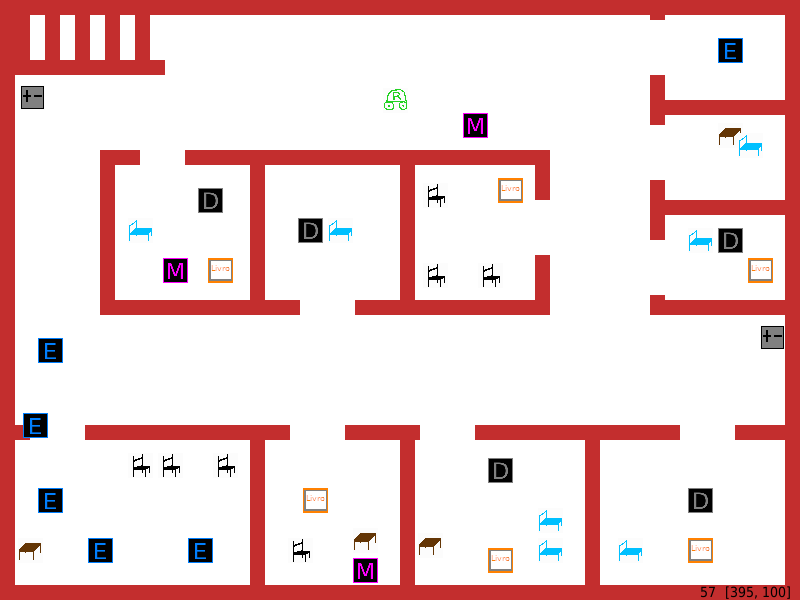
\includegraphics[scale=0.5]{hospital}
    \caption[Mundo utilizado para implementação do projeto]{Mundo virtual original utilizado para a implementação do projeto.}
    \label{fig::hospital}
\end{figure}

A solução passou então pela substituição da matriz por uma estrutura de dados que permite representar de forma bastante eficiente os dados recolhidos sobre o mundo virtual: grafos. Para este fim, foi utilizada a biblioteca \emph{NetworkX} \cite{NetworkX} para a criação e gestão dos mesmos. Dois grafos foram utilizados neste âmbito:

\begin{enumerate}
	\item Grafo \emph{floor} (Figura \ref{fig::grafo_floor}) --- armazena informações sobre as salas visitadas, a sua ligação e os objetos nelas contidos;
	
	\item Grafo \emph{map} (Figura \ref{fig::grafo_map}) --- realiza o mapeamento do mundo, ao registar em detalhe todos os caminhos possíveis entre salas e as portas que as conectam, para efeitos de execução do algoritmo de \textit{path-finding} A*.
\end{enumerate}

\begin{figure}[!htb]
	% TODO: Pôr imagem do grafo floor
	\centering
	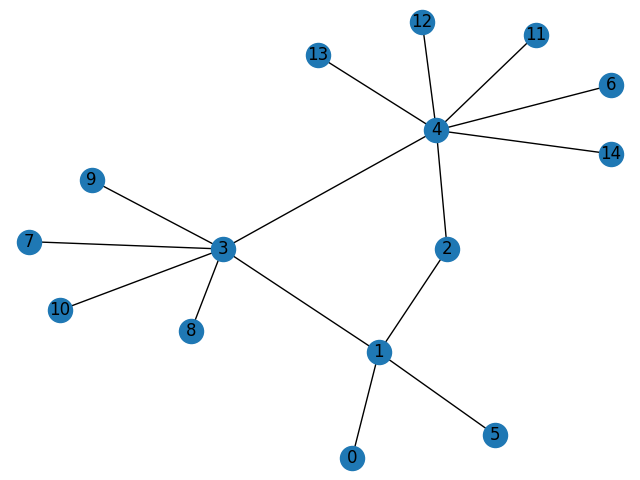
\includegraphics[width=\textwidth]{floor}
	\caption[Grafo \textit{floor}]{Grafo \textit{floor}: cada nodo representa uma divisão visitada pelo \textit{robot} e cada aresta indica que existe uma porta entre os nodos que ela conecta.\\ Este grafo representa o mapa total original fornecido para o projeto.}
	\label{fig::grafo_floor}
\end{figure}

Por análise do grafo da Figura \ref{fig::grafo_floor}, podemos constatar que se trata de um grafo não dirigido, composto por nodos e arestas, sendo que os nodos guardam informações acerca das divisões e como seus atributos constam os objetos contidos nessas mesmas divisões. Os atributos estão definidos como um dicionário, onde a chave do mesmo é a categoria de objeto e o valor é a lista de nomes dos objetos dessa categoria encontrados pelo \emph{robot}.

\begin{figure}[!htb]
	% TODO: Pôr imagem do grafo map
	\centering
	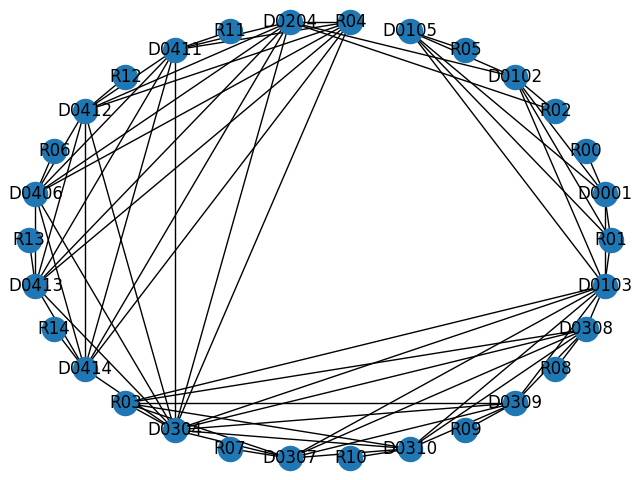
\includegraphics[width=\textwidth]{map}
	\caption[Grafo \textit{map}]{Grafo \textit{map}: cada nodo representa uma divisão visitada pelo \textit{robot} (codificado com \texttt{R}) e uma porta que conecta duas divisões (codificado com \texttt{D}).\\ As ligações diretas entre portas permitem determinar caminhos mais curtos sem passar pelo ponto médio de cada divisão.\\ Este grafo representa o mapa total original fornecido para o projeto.}
	\label{fig::grafo_map}
\end{figure}

Por seu turno, o grafo da Figura \ref{fig::grafo_map}, sendo na mesma um grafo não dirigido, armazena em cada nodo a posição das salas visitadas (i.e. o ponto médio de cada sala) e das portas que conectam as salas em tuplos do tipo $(x, y)$, e em cada aresta é dado como atributo a distância euclidiana entre os dois nodos que esta conecta.

% No decorrer de todo o projeto foi utilizado um modo de \emph{debugging} com \emph{logs} para efeitos de maior facilidade na correção de erros no código.

Em termos de organização do código-fonte do trabalho prático, optou-se por se utilizar classes, as quais se enumeram seguidamente:

\begin{enumerate}
	\item \emph{Log} --- útil para efeitos de \emph{debugging} de forma a identificar mais facilmente possíveis \emph{bugs};
	
	\item \emph{LinearFunction} --- permite criar instâncias de funções lineares necessárias para a resposta às perguntas 5 e 6 (subsecções \ref{ssec::implement:details:perg5} e \ref{ssec::implement:details:perg6}, respetivamente);
	
	\item \emph{Things} --- armazena listas de objetos e pessoas, tratando diretamente da resposta à pergunta 1 (subsecção \ref{ssec::implement:details:perg1}) e auxiliando as restantes classes a gerir os seus dados;
	
	\item \emph{Robot} --- realiza a gestão dos dados inerentes ao \textit{robot}, em particular a velocidade e a bateria, bem como a sua relação com o tempo;
	
	\item \emph{Hospital} --- principal classe do programa na qual a informação relativa ao piso do hospital é atualizada conforme as informações dadas pelo \emph{robot};
	
	\item \emph{Utils} --- coleta um conjunto de funções auxiliares, como por exemplo o cálculo de distâncias, a troca de variáveis e a descrição textual de caminhos.
\end{enumerate}


\section{Detalhes de Implementação}
\label{sec::implement:details}

Nesta secção são descritos os detalhes de implementação para cada pergunta proposta no enunciado do projeto prático, através da explicação dos respetivos algoritmos.


\subsection{Pergunta 1}
\label{ssec::implement:details:perg1}

\enunciado{Qual foi a penúltima pessoa que viste?}

A classe \textit{Things} fornece o método \texttt{getLastButOnePerson()}, o qual devolve o nome da penúltima pessoa que o \textit{robot} encontrou. Este método depende da prévia invocação da função \texttt{add()} por parte da classe \textit{Hospital} a fim de atualizar corretamente as pessoas encontradas.

Caso o \textit{robot} não tenha encontrado pelo menos duas pessoas no momento da pergunta, é devolvida uma mensagem pré-definida de erro pela seguinte constante:

\mintinline[breaklines]{python}{ERROR_NOT_ENOUGH_PEOPLE = "Não foram encontradas pelo menos 2 pessoas até ao momento"}


\subsection{Pergunta 2}
\label{ssec::implement:details:perg2}

\enunciado{Em que tipo de sala estás agora?}

A classe \textit{Hospital} providencia a função \texttt{getCurrentTypeOfRoom()}, o qual devolve um código que indica o tipo da sala onde o \textit{robot} se encontra no momento. Esta função encapsula a utilização de outra: a função \texttt{getTypeOfRoom()}, a qual permite determinar o tipo de qualquer sala a qualquer momento. Neste caso, a primeira função encontra-se definida da seguinte forma:

\begin{minted}[breaklines,linenos]{python}
@staticmethod
def getCurrentTypeOfRoom():
    return Hospital.getTypeOfRoom(Hospital._currentRoom)
\end{minted}

O método \texttt{roomDescription()} converte o código devolvido pelas funções anteriores em descrições textuais a fim de produzir o \textit{output} pretendido.

De notar que a função \texttt{getTypeOfRoom()} determina o tipo da sala com o seguinte algoritmo:

\begin{enumerate}
    \item Se o número da sala está no intervalo $[1, 4]$, então devolve o código correspondente a um corredor;
    \item Para cada atributo do nodo da sala atual, é feita a contagem de cada tipo de objeto que seja mobília (cama, cadeira e mesa);
    \item A contagem dos objetos de cada categoria indica o respetivo tipo de sala:
    \begin{itemize}
        \item Quarto: $\geq$ 1 cama;
        \item Sala de enfermeiros: 0 camas, $\geq$ 1 cadeiras \textbf{e} $\geq$ 1 mesas;
        \item Sala de espera: $>$ 2 cadeiras, 0 mesas, 0 camas.
    \end{itemize}
\end{enumerate}


\subsection{Pergunta 3}
\label{ssec::implement:details:perg3}

\enunciado{Qual o caminho até à sala de enfermeiros mais próxima?}

Para esta pergunta, o método \texttt{getPathToNearestNurseOffice()} da classe \textit{Hospital} devolve uma lista com o nome dos nodos do grafo \textit{map} correspondentes ao caminho mais curto desde a posição atual do \textit{robot} até à sala de enfermeiros mais próxima.

Para este fim, o \textit{robot} é temporariamente adicionado ao grafo \textit{map} e são feitas as ligações por arestas a todos os vizinhos do nodo correspondente à sala onde o \textit{robot} se encontra. De seguida, o algoritmo A* é aplicado sobre o grafo recorrendo aos métodos \texttt{astar\_path} e \texttt{astar\_path\_length} da biblioteca \textit{NetworkX} para todas as salas de enfermeiros conhecidas até ao momento. O caminho mais curto de todos os caminhos determinados corresponde ao caminho para a sala de enfermeiros mais próxima, sendo então este caminho codificado numa lista, a qual é devolvida.

O método \texttt{pathDescription()} da classe \textit{Utils} converte esta lista numa série de instruções em português para fácil leitura do utilizador.


\subsection{Pergunta 4}
\label{ssec::implement:details:perg4}

\enunciado{Qual é a distância até ao médico mais próximo?}

Para esta questão, não tendo sido pedido o caminho, optou-se por se procurar o médico mais próximo em linha reta. A função \texttt{getDistanceToNearestDoctor()} da classe \textit{Hospital} providencia a resposta.

Desta forma, o grafo \textit{floor} é filtrado de forma a recolher os médicos até então encontrados e as respetivas posições. A lista resultante é então mapeada com a função \texttt{distance()} da classe \textit{Utils} de forma a converter as posições dos médicos em distâncias euclidianas em relação ao \textit{robot}. A lista é ordenada pela distância, sendo então devolvido o primeiro elemento desta, correspondente ao médico mais próximo.

A informação é devolvida com o seguinte formato: ``Médico \textit{<nome>} na sala \textit{<n\textordmasculine~da sala>} a uma distância de \textit{<distância>}.''


\subsection{Pergunta 5}
\label{ssec::implement:details:perg5}

\enunciado{Quanto tempo achas que demoras a ir de onde estás até às escadas?}

A resposta a esta pergunta assemelha-se à da pergunta 3 (secção \ref{ssec::implement:details:perg3}), sendo tratada pela função \texttt{getTimeToStairs()} da classe \textit{Hospital}. O \textit{robot} é adicionado temporariamente ao grafo \textit{map} e é determinado o caminho mais curto até às escadas (codificada internamente como sendo a sala 0 (zero)).

Com base na distância determinada, é estimado o tempo que demorará a chegar às escadas com recurso ao método \texttt{predictTimeFromDistance()} da classe \textit{Robot}. Esta classe calcula a cada nova posição do \textit{robot} a variação da velocidade ao longo do tempo sob a forma de uma função linear a fim de se poder extrapolar o tempo necessário a percorrer uma certa distância.

A estimativa é feita com a seguinte fórmula:

\begin{equation}
    \Delta t = \frac{2d}{v_f + v_i}
    \label{eq::time_from_distance}
\end{equation}

Esta é determinada com base no seguinte facto físico:

\begin{equation}
    d = \int_{t_i}^{t_f}{v(t)dt}
\end{equation}

A distância é, portanto, a área sob a curva da função $v(t)$ (velocidade em função do tempo). Todavia, no nosso caso, a ``curva'' é uma reta uma vez que se optou por usar funções lineares para maior eficiência.

\begin{figure}[!hbtp]
    \centering
    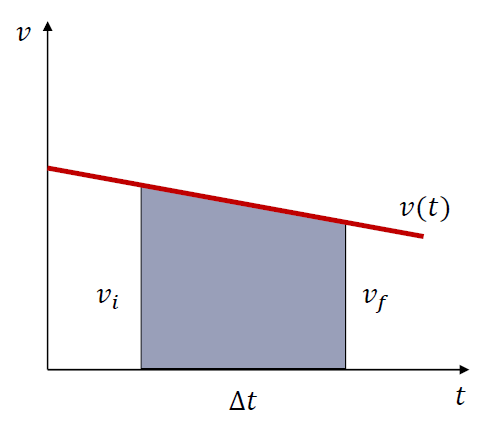
\includegraphics[scale=0.5]{fun-vt}
    \caption[Estimativa da velocidade do \textit{robot}: função $v(t)$]{Estimativa da velocidade do \textit{robot}: função $v(t)$.}
    \label{fig::fun_vt}
\end{figure}

Desta forma, a área sob a curva é a área de um trapézio (Figura \ref{fig::fun_vt}), tal que:

\begin{equation}
    d = \frac{v_f + v_i}{2}\Delta t
\end{equation}

Por rearranjo da igualdade, chega-se à equação (\ref{eq::time_from_distance}).

O tempo determinado é formatado pela função \texttt{timeToStr()} da classe \textit{Utils} de forma a apresentar a estimativa em segundos e milissegundos.



\subsection{Pergunta 6}
\label{ssec::implement:details:perg6}

\enunciado{Quanto tempo achas que falta até ficares sem bateria?}

À semelhança da questão 5 (secção \ref{ssec::implement:details:perg5}), a classe \textit{Robot} avalia a variação da bateria ao longo do tempo com uma função linear.

O método \texttt{getTimeToDie()} da classe \textit{Hospital}, utilizada para responder a esta pergunta, encapsula o método \texttt{predictTimeFromBattery()} da classe \textit{Robot}, pedindo o tempo que falta até a bateria chegar a \SI{0}{\percent}.

Novamente, o método \texttt{timeToStr()} da classe \textit{Utils} é utilizado para converter o número obtido em segundos e milissegundos.


\subsection{Pergunta 7}
\label{ssec::implement:details:perg7}

\enunciado{Qual a probabilidade de encontrar um livro numa divisão se já encontraste uma cadeira?}

Para responder a esta pergunta, tomámos particular atenção ao seguinte excerto do enunciado do projeto:

\begin{quote}
    \itshape A existência de uma cama, torna mais provável que exista um livro na mesma divisão. O mesmo se passa com a existência de uma cadeira: aumenta a probabilidade de existirem livros na mesma divisão.
\end{quote}

Tal significa que os eventos \textbf{não são independentes}, o que invalida por princípio a aplicação direta de uma probabilidade condicionada. Neste sentido, optou-se por uma \textbf{probabilidade condicionada baseada numa Rede \textit{Bayesiana}} (Figura \ref{fig::bayes}).

\begin{figure}[!htbp]
    \centering
    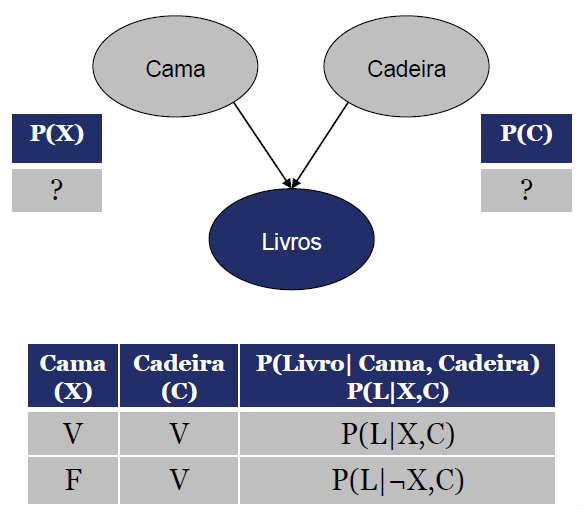
\includegraphics[scale=0.6]{bayes}
    \caption[Rede \textit{Bayesiana} para a pergunta 7]{Rede \textit{Bayesiana} que correlaciona os seguintes eventos: sala conter camas, sala conter cadeiras e sala conter livros.}
    \label{fig::bayes}
\end{figure}

Seja então:
\begin{itemize}[nosep]
    \item $L$: Livro
    \item $C$: Cadeira
    \item $X$: Cama
\end{itemize}

Com base nesta Rede \textit{Bayesiana}, sabemos que a probabilidade procurada é a seguinte:

\begin{equation}
    P(L|C) = \frac{P(L,C)}{P(C)}
\end{equation}

A probabilidade $P(C)$ pode ser determinada diretamente pela divisão entre o número de salas com cadeiras e o número total de salas (que não corredores). Contudo, a probabilidade $P(L,C)$ é dada pela equação (\ref{eq::prob_lc}).

\begin{equation}
    P(L,C) = \sum_{X \in \{V,F\}}{P(C,X,L)} = P(C,X,L) + P(C,\neg X,L)
    \label{eq::prob_lc}
\end{equation}

Por conseguinte, as duas probabilidades necessárias são dadas pela respetiva marginalização:
\begin{itemize}
    \item $P(C,X,L) = P(X)P(C)P(L|X,C)$;
    \item $P(C,\neg X,L) = P(\neg X)P(C)P(L|\neg X,C)$.
\end{itemize}

Onde $P(\neg X) = 1-P(X)$.

Por fim, temos que:
\begin{itemize}
    \item $P(L|X,C) = \frac{P(L \wedge X \wedge C)}{P(X \wedge C)}$;
    \item $P(L|\neg X,C) = \frac{P(L \wedge \neg X \wedge C)}{P(\neg X \wedge C)}$.
\end{itemize}

Estas últimas podem ser determinadas diretamente contabilizando os números das salas totais e das salas que cumprem cada uma das condições pretendidas (por exemplo, $P(X \wedge C) = (\mathrm{salas~com~X~e~C}) / (\mathrm{total~salas})$).

O método \texttt{getProbabilityOfBookIfChairFound()} da classe \textit{Hospital} realiza esta série de cálculos a fim de encontrar uma solução à equação (\ref{eq::prob_lc}).


\subsection{Pergunta 8}
\label{ssec::implement:details:perg8}

\enunciado{Se encontrares um enfermeiro numa divisão, qual é a probabilidade de estar lá um doente?}

Por falta de indicação em contrário no enunciado do projeto, consideramos que estes são eventos \textbf{independentes}, pelo que pode ser aplicada a \textbf{probabilidade condicionada}.

O método \texttt{getProbabilityOfPatientKnowingNurses()} da classe \textit{Hospital} realiza este cálculo, respondendo à equação (\ref{eq::prob_de}):

\begin{equation}
    P(D|E) = \frac{P(D \wedge E)}{P(E)}
    \label{eq::prob_de}
\end{equation}

Onde:
\begin{itemize}[nosep]
    \item $P(D)$: probabilidade de um doente estar numa sala;
    \item $P(E)$: probabilidade de um enfermeiro estar numa sala.
\end{itemize}

Tendo em conta que, por exemplo, $P(E) = (\mathrm{salas~com~E}) / (\mathrm{total~salas})$, o cálculo destas probabilidades é direto, sendo por fim retornado o resultado da divisão da equação (\ref{eq::prob_de}).



\section{Conclusões}
\label{sec::implement:conc}

No presente capítulo foram apresentados os passos e os métodos necessários ao desenvolvimento do projeto prático e do funcionamento do mesmo. 

Desta forma, através do conteúdo exposto neste capítulo, encontra-se a apresentação do projeto desenvolvido e o funcionamento do mesmo, mas também a contextualização das ferramentas utilizadas conforme listadas no Capítulo ~\ref{ch::tecno}.